\subsubsection{Fuel savings}\label{sec:fuel-savings}
% 
The lower fuel consumption is one of the main benefit of platooning and one of the main reasons why freight companies would adapt this technology. But in order to convince these companies, there must be clear evidence that platooning really saves fuel. In SARTRE \cite{Chan2012ProjectSARTRE} the CFD (Computational Fluid Dynamic) aerodynamic simulations and real life testing have been done to find it out.
%
\subsubsection*{CFD test}
In CFD tests 5 vehicles were involved, 2 trucks and 3 cars, the order was leading truck, following truck and 3 following cars. Tests were done with different distance between vehicles starting with 3 meters till 15 meters. Here vehicles were perfectly aligned behind each other. Figure \ref{fig:cx-reduction} shows by how many percent the drag of vehicles has been reduced with different distances between them. It seems like the closer vehicles are, the better as the drag reduction (Cx) is higher. From simulation, the best fuel saving distance is 3-4 meters. However, having vehicles so close to each other causes instabilities and therefore the best distance would be 6-8 meters according to SARTRE project \cite[p. 33]{Chan2012ProjectSARTRE}.\par
% 
\begin{figure}[p]
    \centering
    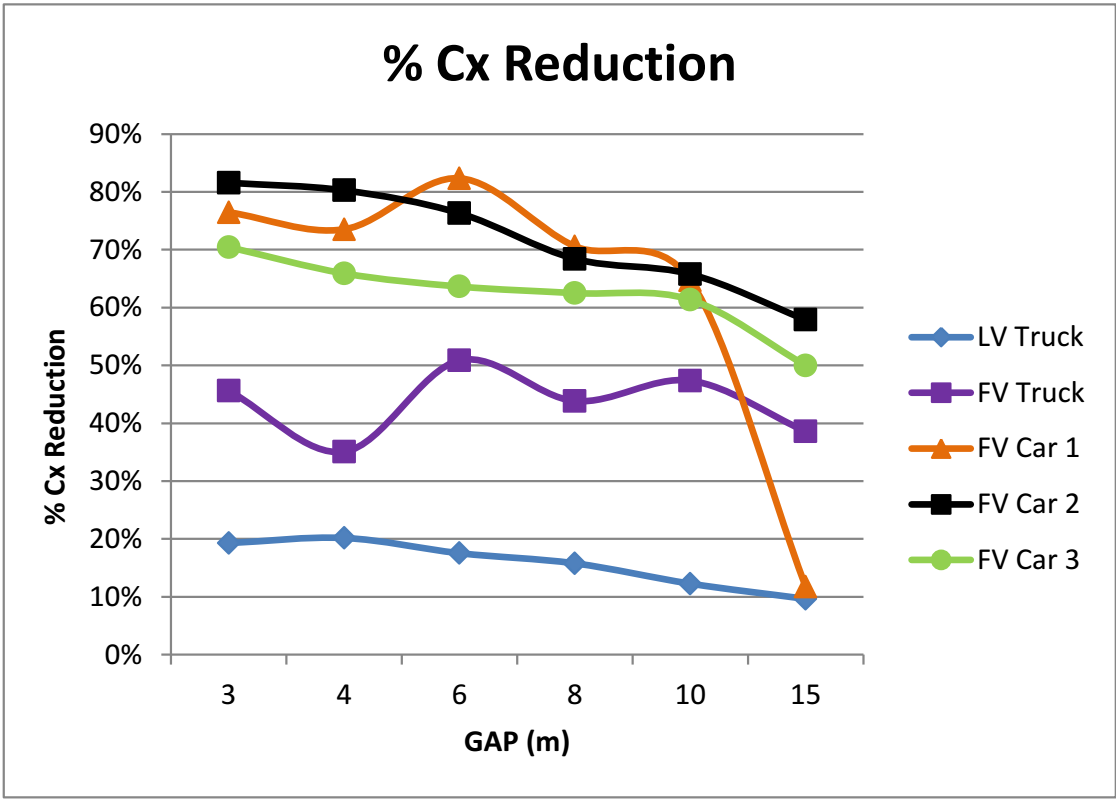
\includegraphics[width=.95\textwidth]{cx-reduction}
    \caption{Drag reduction for platooning vehicles as a function of gap between them. CFD simulation. Taken from \cite{Chan2012ProjectSARTRE}}
    \label{fig:cx-reduction}
\end{figure}
% 
In the test mentioned above the vehicles were perfectly aligned. This however, is very unlikely to happen in real life. Therefore, in the Companion project when making simulation virtually they count with this offset of vehicles and measured difference in drag of 2 truck with different lateral offset, the distance between trucks was 3 meters. The simulated offset was 0.1, 0.25, 0.5 and 1 meter. The Figure \ref{fig:lateral-offset} shows the results of simulations.
% 
\begin{figure}[p]
    \centering
    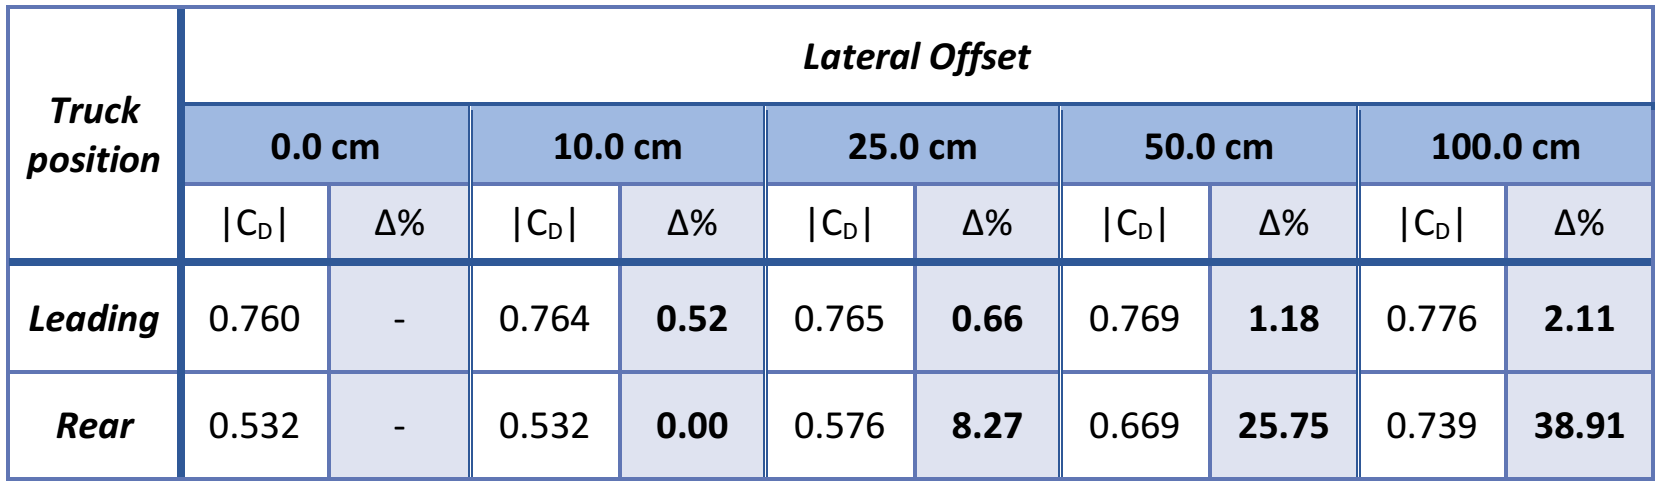
\includegraphics[width=.95\textwidth]{lateral-offset}
    \caption{Difference in drag by lateral offset. CFD simulation. Taken from \cite[p. 19]{Laxhammar2015CooperativeConsumption}}
    \label{fig:lateral-offset}
\end{figure}
% 
As it can be seen in Figure \ref{fig:lateral-offset} small lateral offset of 10 cm does not influence the drag at all, but as the offset is bigger it can be observed that the following truck experiences pretty high values of drag compared to no offset. There is almost 39\% rise in drag when there is 100 cm offset and the drag value of following truck is almost the same as of the leading one. But for leading truck, different offset values did not change much as the maximum drag rise was a bit more than 2\% which is negligible. From this we found that small offset does not have a noticeable impact on the drag but vehicles should be as aligned as possible.\par
%
\begin{figure}[p]
    \centering
    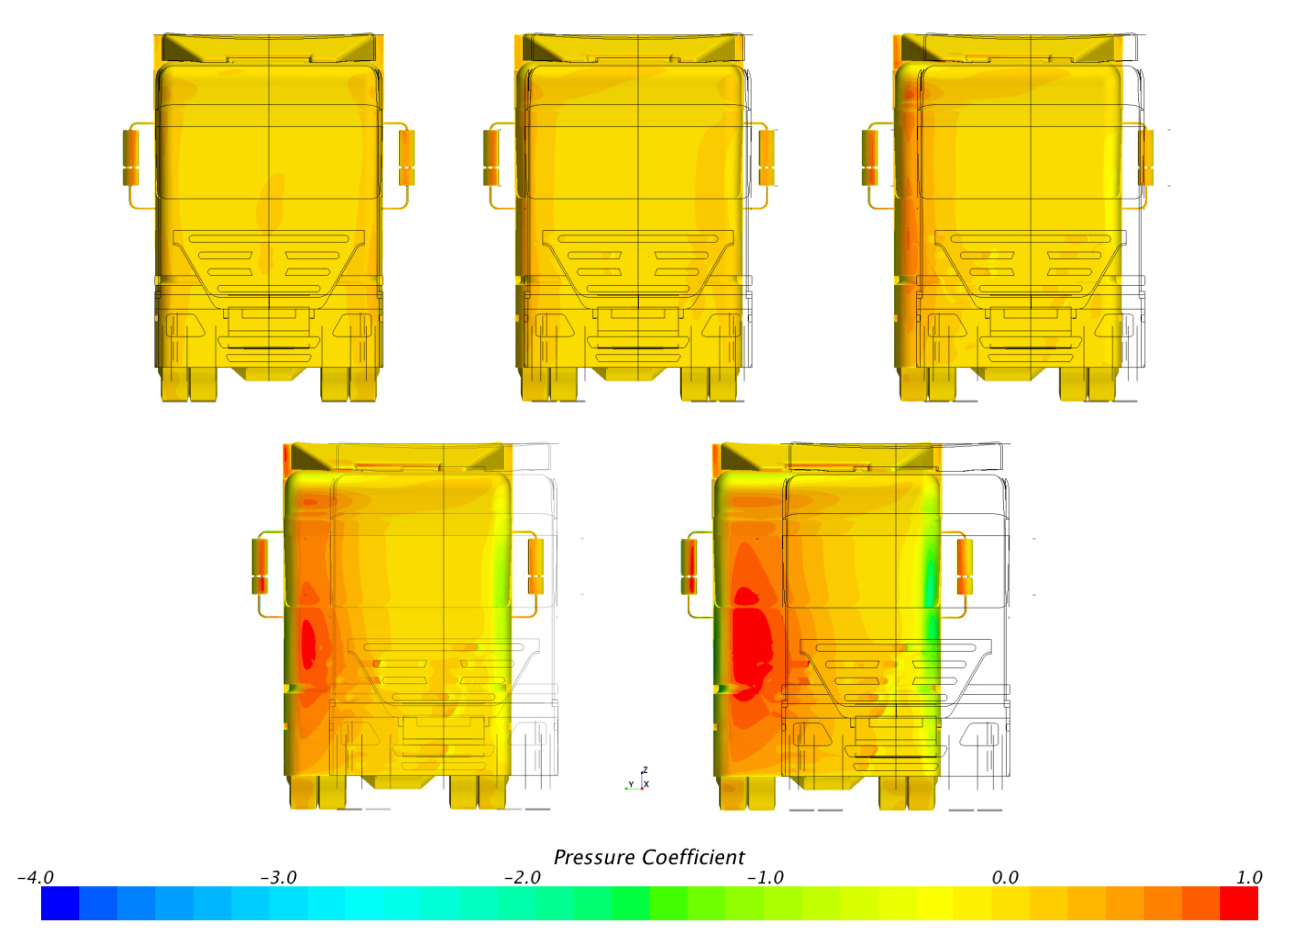
\includegraphics[width=.95\textwidth]{pressure-coef}
    \caption{Pressure on following truck with different offset. CFD simulation. Taken from \cite[p. 19]{Laxhammar2015CooperativeConsumption}}
    \label{fig:pressure-coef}
\end{figure}
% 
% 
\subsubsection*{Real life tests}
In real life tests, a fuel consumption of each vehicle has been first measured separately (not in a platoon) and then in a platoon made up by 2 trucks and 3 cars, the same order as in the CFD simulation. Different distances were tested, starting at 5 meters up to 15 meters. Results are shown in Figure \ref{fig:fuel-savings-full}.\par
% 
As it can be seen in the table, there is a fuel saving effect because of the drag reduction in a platoon in reality as well. The right data could not be measured for cars in distances smaller than 7 meters because of an emergency system which was triggered in cars and made fuel consumption higher. Nonetheless, the graph show that the closer vehicles are the bigger is fuel saving and that also validate that platooning saves fuel.
% 
\begin{figure}[h]
    \centering
    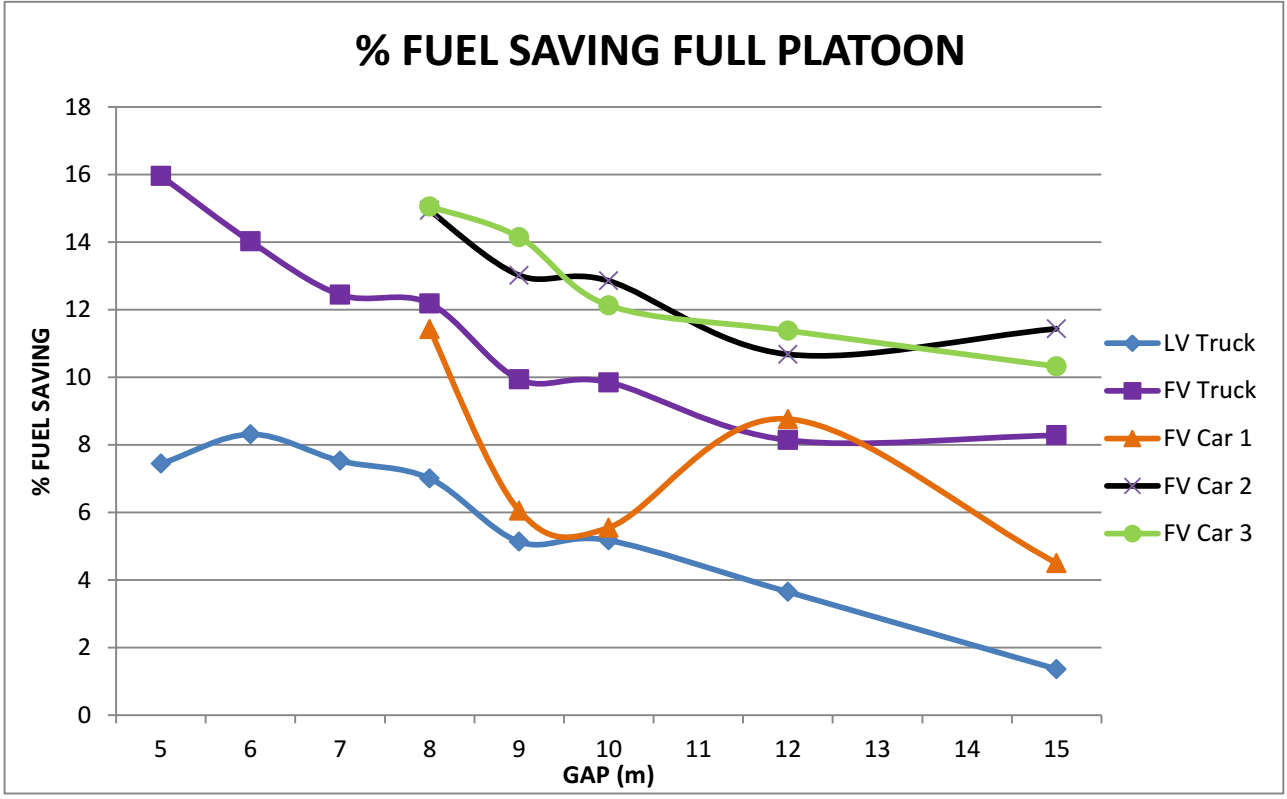
\includegraphics[width=.95\textwidth]{fuel-savings-full}
    \caption{Fuel savings for platooning vehicles. Real-life test. Taken from \cite[p. 36]{Chan2012ProjectSARTRE}.}
    \label{fig:fuel-savings-full}
\end{figure}
% 
